%% Copernicus Publications Manuscript Preparation Template for LaTeX Submissions
%% ---------------------------------
%% This template should be used for copernicus.cls
%% The class file and some style files are bundled in the Copernicus Latex Package, which can be downloaded from the different journal webpages.
%% For further assistance please contact Copernicus Publications at: production@copernicus.org
%% https://publications.copernicus.org/for_authors/manuscript_preparation.html

%% copernicus_rticles_template (flag for rticles template detection - do not remove!)

%% Please use the following documentclass and journal abbreviations for discussion papers and final revised papers.

%% 2-column papers and discussion papers
\documentclass[amt, manuscript]{copernicus}



%% Journal abbreviations (please use the same for preprints and final revised papers)

% Advances in Geosciences (adgeo)
% Advances in Radio Science (ars)
% Advances in Science and Research (asr)
% Advances in Statistical Climatology, Meteorology and Oceanography (ascmo)
% Annales Geophysicae (angeo)
% Archives Animal Breeding (aab)
% Atmospheric Chemistry and Physics (acp)
% Atmospheric Measurement Techniques (amt)
% Biogeosciences (bg)
% Climate of the Past (cp)
% DEUQUA Special Publications (deuquasp)
% Drinking Water Engineering and Science (dwes)
% Earth Surface Dynamics (esurf)
% Earth System Dynamics (esd)
% Earth System Science Data (essd)
% E&G Quaternary Science Journal (egqsj)
% EGUsphere (egusphere) | This is only for EGUsphere preprints submitted without relation to an EGU journal.
% European Journal of Mineralogy (ejm)
% Fossil Record (fr)
% Geochronology (gchron)
% Geographica Helvetica (gh)
% Geoscience Communication (gc)
% Geoscientific Instrumentation, Methods and Data Systems (gi)
% Geoscientific Model Development (gmd)
% History of Geo- and Space Sciences (hgss)
% Hydrology and Earth System Sciences (hess)
% Journal of Bone and Joint Infection (jbji)
% Journal of Micropalaeontology (jm)
% Journal of Sensors and Sensor Systems (jsss)
% Magnetic Resonance (mr)
% Mechanical Sciences (ms)
% Natural Hazards and Earth System Sciences (nhess)
% Nonlinear Processes in Geophysics (npg)
% Ocean Science (os)
% Polarforschung - Journal of the German Society for Polar Research (polf)
% Primate Biology (pb)
% Proceedings of the International Association of Hydrological Sciences (piahs)
% Safety of Nuclear Waste Disposal (sand)
% Scientific Drilling (sd)
% SOIL (soil)
% Solid Earth (se)
% The Cryosphere (tc)
% Weather and Climate Dynamics (wcd)
% Web Ecology (we)
% Wind Energy Science (wes)

% Pandoc citation processing

% The "Technical instructions for LaTex" by Copernicus require _not_ to insert any additional packages.
% 
% tightlist command for lists without linebreak
\providecommand{\tightlist}{%
  \setlength{\itemsep}{0pt}\setlength{\parskip}{0pt}}


%
\begin{document}


\title{On Measuring Sensible-Heat Flux With Airborne Thermometers}


\Author[1]{William}{Cooper}
\Author[1]{Adriana}{Bailey}
\Author[1]{Joshua}{Carnes}


\affil[1]{Earth Observing Laboratory, National Center for Atmospheric
Research 80307-3000 Boulder, CO, United States}

\runningtitle{Measuring Sensible-Heat Flux}

\runningauthor{Cooper}


\correspondence{William\ Cooper\ (cooperw@ucar.edu)}



\received{}
\pubdiscuss{} %% only important for two-stage journals
\revised{}
\accepted{}
\published{}

%% These dates will be inserted by Copernicus Publications during the typesetting process.


\firstpage{1}

\maketitle


\begin{abstract}
Most measurements of temperature from research aircraft rely on sensors
that have inadequate response for demanding applications, including
especially measuring the flux density of sensible heat. In order to
improve that measurement, this paper uses in-flight measurements to
determine the frequency-domain transfer function that characterizes the
time response of standard airborne temperature sensors, with emphasis on
the ``fast'' Rosemount unheated sensor. Airborne thermometers sense the
``recovery temperature'' produced when air is compressed on approach to
the sensor. The change in temperature produced by that compression,
termed ``dynamic heating'' in this paper, fluctuates as the airspeed
changes, and those changes in airspeed are measured so the expected
fluctuations in recovery temperature are known. In this study, flight
segments were used where such turbulent fluctuations were the dominant
cause of fluctuations in the recovery temperature so that the sensor
response could be used to find the transfer function. Examples and a
simulation illustrate that, without correction, measurements of
sensible-heat flux with a standard sensor can be more than 30\% too low,
while the proposed correction procedure removes this error. An
additional result of the study is the identification of a source of
error, prevalent in most archived temperature measurements from research
aircraft, that results when conventional treatments of dynamic heating
do not take into account the time response of the sensor.
\end{abstract}




\newpage

\introduction[Introduction]

Research aircraft routinely measure air temperature, but standard
sensors do not respond fast enough to meet many scientific needs. In
particular, measurements of the flux of sensible heat require faster
response than is typically available, as do measurements of
near-discontinuous changes such as those at the top of boundary layers
or at cloud boundaries. The eddy-correlation measurement of the flux
density of sensible heat (\(F_{s}\)) is conventionally evaluated from
the mean value of this expression (c.f., e.g., \citet{hartmann201695}):
\begin{equation}
F_{s}=\rho_{a}\thinspace C_{p}\left\langle w^{\prime}T^{\prime}\right\rangle \label{eq:heatFlux}
\end{equation} where \(\rho_{a}\) is the density of air, \(C_{p}\) the
specific heat of air at constant pressure, \(w\) the vertical wind, and
\(T\) the temperature. Primes in this equation denote fluctuations from
the mean and angle brackets denote an ensemble average. This measurement
thus requires that temperature be measured with sufficient response to
resolve the eddy sizes that make significant contributions to the flux.
(Additional information regarding measuring fluxes by eddy correlation
is contained in, e.g., \citet{lenschow95micro}.)

\citet{FrieheKhelif1992} suggested that 4--5\unit{\,Hz} is ``just
adequate'' (for flight at around \unit{125\,m\,s^{-1}}) and that
\unit{25\,Hz} would be desirable. If the response of the temperature
sensor is incomplete or shifted in phase at a particular frequency, an
error will be introduced into the measurement of sensible-heat flux. To
avoid significant errors, it therefore is essential to characterize the
time response of the temperature sensor used and, where necessary, to
apply corrections to compensate for that response.

\section{\texorpdfstring{Determining the Transfer Function
\label{sec:theTransferFn}}{Determining the Transfer Function }}

The time response of an airborne thermometer can be characterized by a
frequency-domain transfer function that relates the measurement (the
sensor output) to the measurand (the temperature). This section presents
the transfer functions for some standard sensors. Two coupled
differential equations with three parameters are proposed as the basis
for this characterization, but the frequency-domain transfer function is
determined independent of those equations. When the equations predict a
transfer function matching the observations, they provide a useful
generalization. Furthermore, the parameters in those equations can be
constrained with low uncertainty by fitting to the observed transfer
functions. The transfer functions then are used in the sections that
follow to access how measurements of temperature are affected.

Because airborne thermometers respond to the temperature of the air
after it is compressed upon entering the sensor housing, the measurand
is the ``recovery temperature'' (\(T_{r}\)), which exceeds the ambient
air temperature (\(T_{a}\)) by the amount of dynamic heating (\(Q\)):
\begin{equation}
T_{r}=T_{a}+Q\,\,\,.{\label{eq:recoveryTemperature}}
\end{equation} The transfer functions determined in this section apply
to the recovery temperature rather than the calculated air temperature
after correction for dynamic heating. In this regard, this study differs
from earlier ones. The justification, developed in later sections, is
that this approach is required so that the correction for dynamic
heating can be applied with proper treatment of the sensor response.

\subsection{\texorpdfstring{Theory \label{subsec:Theory}}{Theory }}

Previous studies have demonstrated that a simple first-order exponential
equation with one time constant does not represent the time response of
many standard temperature sensors used on research aircraft. The
suggested explanation \citep{NCAR_OpenSky_TECH-NOTE-000-000-000-064} is
that heat is transferred to the sensing wire of those sensors not only
from the air but also from the supporting structure that is in contact
with the wire. \citet{FrieheKhelif1992}, following other prior work
including that of \citet{rodi1972analysis} and
\citet{mccarthy1973method}, suggested representing the response with two
time constants:
\begin{equation}\Theta(t)=A_{1}e^{-t/\tau_{1}}+A_{2}e^{-t/\tau_{2}}{\label{eq:FrieheKhelif}}
\end{equation} where \(\Theta(t)\) is the normalized history of the
measured temperature decaying from an initial value of one to a final
value of zero. The sum of the coefficients \(A_{1}\) and \(A_{2}\) must
then be one. The values for \{\(A_{1},\,A_{2},\,\tau_{1},\,\tau_{2}\)\}
suggested by \citet{FrieheKhelif1992} for an unheated Rosemount 102E4AL
sensor were \{0.65, 0.35, \unit{0.09\,s}, \unit{0.5\,s}\}.

This work, following the approach of \citet{PayneEtAl1994}, represents
the time response of the sensor by two coupled differential equations,
one that describes the response of the support on which the sensing wire
is wound to the air temperature and a second that describes the response
of the sensing wire to two inputs, one from the support and one from the
air. No attempt is made here to determine the parameters from first
principles as in \citet{PayneEtAl1994}, however; instead, parameters
entering the equations are determined empirically. The equations are:
\begin{align}
\frac{dT_{s}(t)}{dt} & =\frac{T_{r}(t)-T_{s}(t)}{\tau_{2}}{\label{eq:Ts}} \\
\frac{dT_{m}(t)}{dt} & =\frac{a(T_{r}(t)-T_{m}(t))+(1-a)(T_{s}(t)-T_{m}(t))}{\tau_{1}}\nonumber\\
& = \frac{\left\{ aT_{r}(t)+(1-a)T_{s}(t)\right\} -T_{m}(t)}{\tau_{1}}{\label{eq:Tm}}
\end{align} where \(T_{s}(t)\) is the temperature of the
\uline{s}upport, \(T_{m}(t)\) the \uline{m}easured temperature of the
sensing wire, and \(T_{r}(t)\) the true \uline{r}ecovery temperature
that is the measurand. For heat transfer to or from the wire, the
parameter \(a\) then represents the fraction of the heat transferred by
the air, while the fraction \((1-a)\) is transferred to or from the
support. The wire responds to the combined transfers of heat with
characteristic time constant \(\tau_{1}\) while the support structure
responds to the air temperature more slowly, with time constant
\(\tau_{2}\). It is straightforward to apply Eq.~\eqref{eq:Ts} and
Eq.~\eqref{eq:Tm} to changing but not necessarily discrete conditions,
so a general response to a given air-temperature history can be
predicted by numerical integration of these equations. Furthermore, the
equations are linear and, for constant values of the parameters, they
are also time-invariant (i.e., ``LTI'') descriptions of the response. As
a result, a particular signal for \(T_{r}(t)\) can be decomposed into
its sinusoidal Fourier components and each will satisfy these equations
independently.

The first equation does not involve the measurement, so for a particular
history of recovery temperature \(T_{r}(t)\) the support temperature can
be determined solely by integration of Eq.~\eqref{eq:Ts}. Then, with
\(T_{s}(t)\) determined, Eq.~\eqref{eq:Tm} can be integrated to find the
expected measurement \(T_{m}(t)\) for a specified measurand history
\(T_{r}(t)\). The inverse process, finding \(T_{r}(t)\) from the
measurements \(T_{m}(t)\), is also straightforward and only slightly
more complicated, as discussed in
Appendix~\ref{sec:Correcting-the-Temperature}. These equations have
analytic solutions that are sinusoidal functions if the measurand is
sinusoidal. For example, if the actual recovery temperature is
\(T_{r}(t)=\sin\omega t\) where \(\omega\) is the angular frequency,
then the solutions for \(T_{s}(t)\) and \(T_{m}(t)\) are given by the
following equations: \begin{align}
T_{s}(t)= & b\sin(\omega t+\zeta){\label{eq:TsSolved}} \\
T_{m}(t)= & c\sin(\omega t+\phi)=C_{1}\cos\omega t+C_{2}\sin\omega t{\label{eq:TmSolved}}
\end{align} where \(b=(1+\omega^2\tau_2^2)^{-1/2}\),
~\(\zeta=-\arctan(\omega\tau_2)\), and the amplitude and phase of the
response are given by \begin{align}
c= & \sqrt{C_{1}^{2}+C_{2}^{2}}{\label{eq:responseAmp}} \\
\phi= & \arctan(C_{1}/C_{2}){\label{eq:responsePhase}}
\end{align} with \begin{align}
C_{1}= & \frac{-\omega}{(1+\omega^{2}\tau_{1}^{2})}\left(\tau_{1}a+\frac{(1-a)(\tau_{1}+\tau_{2})}{(1+\omega^{2}\tau_{2}^{2})}\right){\label{eq:C1}} \\
C_{2}= & \left(\frac{1}{1+\omega^{2}\tau_{1}^{2}}\right)\left(a+\frac{(1-a)(1-\omega^{2}\tau_{1}\tau_{2})}{(1+\omega^{2}\tau_{2}^{2})}\right){\label{eq:C2}}
\end{align}

\citet{mccarthy1973method} used the derivative of the step-function
response (Eq.~\eqref{eq:FrieheKhelif}) to find the impulse response
function and, from its Fourier transform, the sensor transfer function.
That leads to the following alternate expressions for \(C_{1}\) and
\(C_{2}\): \begin{align}
C_{1}= & -\omega\left(\frac{A_{1}\tau_{1}}{1+\omega^{2}\tau_{1}^{2}}+\frac{A_{2}\tau_{2}}{1+\omega^{2}\tau_{2}^{2}}\right){\label{eq:C1M}} \\
C_{2}= & \left(\frac{A_{1}}{1+\omega^{2}\tau_{1}^{2}}+\frac{A_{2}}{1+\omega^{2}\tau_{2}^{2}}\right){\label{eq:C2M}}
\end{align} With \(A_{2}=(1-a)/(1-\tau_{1}/\tau_{2})\) and
\(A_{1}=1-A_{2},\) these are equivalent to the expressions for the same
coefficients given by Eq.~\eqref{eq:C1} and Eq.~\eqref{eq:C2}. This
demonstrates that Eq.~\eqref{eq:Ts} and Eq.~\eqref{eq:Tm} are consistent
with the step-function response given by Eq.~\eqref{eq:FrieheKhelif} and
with the equations used by \citet{mccarthy1973method} and
\citet{InverarityJTech2000}, among others.

The transfer function \(H(\omega)=c(\omega)e^{i\phi(\omega)}\) then
characterizes how the sensor will respond to a unit-amplitude sine wave
with angular frequency \(\omega=2\pi\nu\) where \(\nu\) is the
frequency. For a particular set of parameters (\(a\)=0.733,
\(\tau_{1}\)=0.0308\unit{\,s}, \(\tau_{2}\)=0.447\unit{\,s}),
characteristic of an unheated Rosemount 102E4AL sensor (hereafter called
the ``unheated sensor''), the amplitude response and phase delay of the
transfer function are shown in Fig.~\ref{fig:LTsolution}. Similar plots
of the amplitude (but not the phase) have been shown by
\citet{mccarthy1973method} and \citet{nicholls1978measurements}.
Modified transfer functions for two small changes to these parameters
are also shown to illustrate the sensitivity of the solution to these
parameters. This figure illustrates that serious errors will enter
estimates of the sensible heat flux if temperature fluctuations at
frequencies above \unit{1\,Hz} make a significant contribution to the
flux. The contribution to the cospectrum of temperature and vertical
wind will be reduced by the product of the amplitude and the cosine of
the phase such that at \unit{10\,Hz} the error is about 86\%, but even
at \unit{1\,Hz} the error is about 28\%.

\begin{figure}

\begin{center}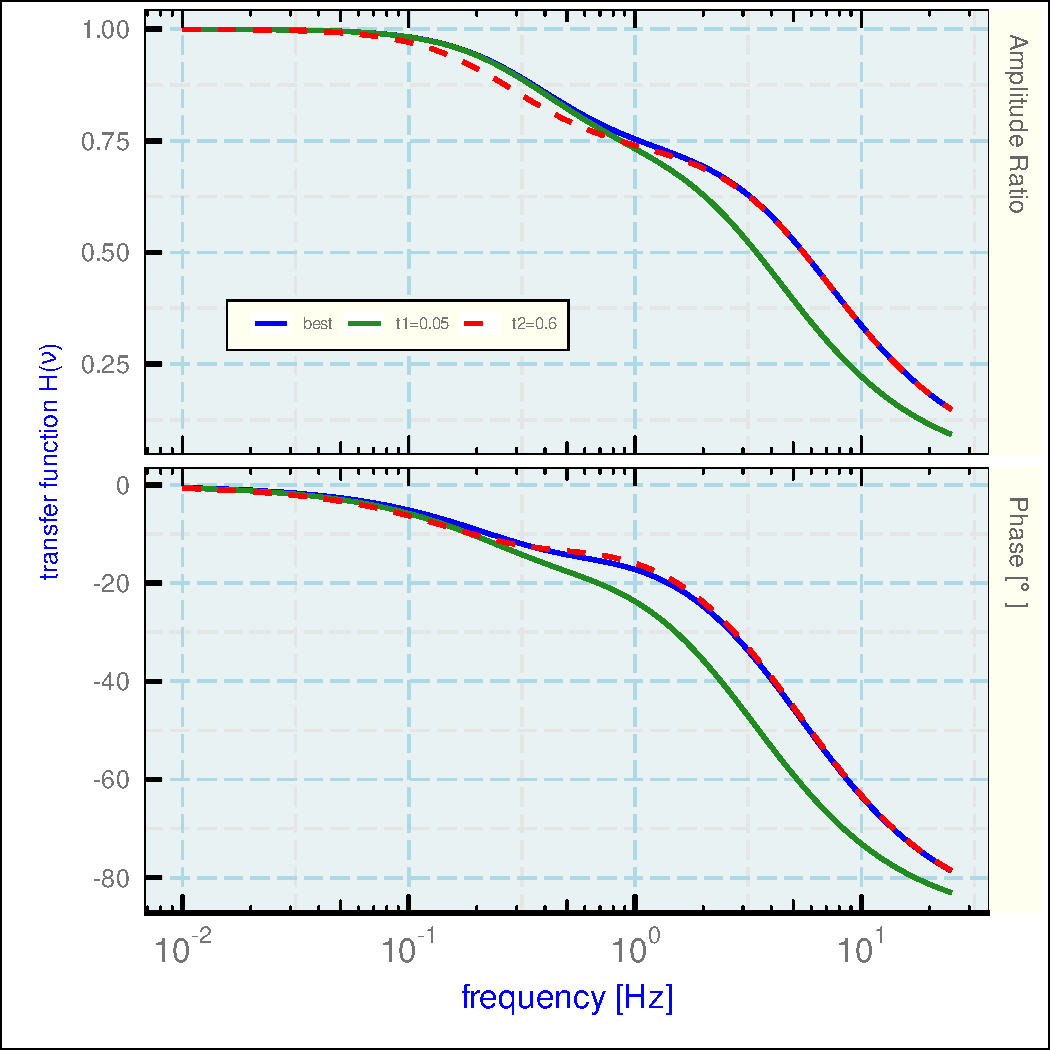
\includegraphics[width=8.3cm]{figure/fig1} \end{center}
\caption{The amplitude ratio (gain) and phase for the frequency-domain transfer function of an unheated temperature sensor. The parameters representing that sensor, labelled "best," are $a$=0.733, $\tau_1$=\unit{0.0308\,s} and $\tau_2$=\unit{0.447\,s}. To illustrate sensitivity,  the curves labelled "t1=0.05" and "t2=0.6" use instead $\tau_1$=\unit{0.05\,s} and $\tau_2$=\unit{0.6\,s}, respectively.\label{fig:LTsolution}}
\end{figure}

These equations and their solution provide a basis for correcting either
the measured temperature or the sensible-heat flux calculated from the
cospectrum in Eq.~\eqref{eq:heatFlux}. Corrected values can be obtained
by several methods including integration of the equations for the
derivatives (Eqs.~\eqref{eq:Ts} and \eqref{eq:Tm}) or by dividing the
Fourier transform of the time series by the transfer function and then
using inverse Fourier transformation to recover the corrected time
series. Those correction schemes are discussed in Appendix~A. To support
such corrections, the next section determines the transfer function
experimentally.

\subsection{\texorpdfstring{The response to dynamic
heating\label{subsec:Dynamic-heating}}{The response to dynamic heating}}

The evaluation of the time response that follows uses the fluctuations
in dynamic heating produced by airspeed fluctuations. These fluctuations
are often significantly larger than real fluctuations in the ambient
temperature. \citet{BangeEtAl2013.ch2} (cf.~their Eq.~2.23) give the
relationship between dynamic heating (\(Q\)) and measurable quantities
as the second equality in the following equation: \begin{equation}
Q=\alpha_{r}\frac{V^{2}}{2C_{p}}=T_{r}\left(\frac{\alpha_{r}M^{2}R_{a}/(2C_{v})}{1+\alpha_{r}M^{2}R_{a}/(2C_{v})}\right){\label{eq:DHterm}}
\end{equation} where \(\alpha_{r}\) is the ``recovery factor''
characterizing the extent to which the air is brought to rest relative
to the sensor, \(V\) is the airspeed, \(C_{p}\) and \(C_{v}\) are
respectively the specific heat of air at constant pressure and constant
volume. \(T_{r}\) is the recovery temperature expressed in absolute
units, \(M\) the Mach number, and \(R_{a}\) the gas constant for air.
Because dynamic heating can exceed \unit{25^{\circ}C} at jet-aircraft
flight speeds, it is often the dominant cause of fluctuations in the
recovery temperature. If the fluctuations in dynamic heating are higher
in frequency than those to which the sensor can respond, corresponding
fluctuations will be attenuated in the measured spectrum and the phase
of the response relative to the imposed signal will vary, from near
\(0^{\circ}\) for fluctuations slow compared to sensor response to near
or above \(90^{\circ}\) for fast fluctuations. The amplitude and phase
of the measured recovery temperature relative to the forcing from
dynamic heating therefore can be used as sensitive indicators of the
response characteristics of the sensor and can constrain parameters like
\(a\), \(\tau_{1}\) and \(\tau_{2}\) that fit the differential equations
to the observations. The evaluation in terms of the amplitude ratio and
phase shift of the recovery temperature in response to dynamic heating
will be used to characterize the transfer function and to determine if
it is represented adequately by the parameterized form given by
Eq.~\eqref{eq:responseAmp} and Eq.~\eqref{eq:responsePhase}.

\subsection{Data sources}

The present investigation uses measurements from two NSF/NCAR (National
Science Foundation / National Center for Atmospheric Research) research
aircraft, a Gulfstream V (hereafter, GV) and a Hercules C-130. The
temperature sensors producing the measurements are in widespread use so
these results should have broad applicability. Some aspects of the
uncertainty limits associated with these measurements of temperature are
included in an NCAR Technical Note \citep{cooper2016ncartn}, where it
was estimated that the standard uncertainty in measurements of
temperature from the GV is about \unit{0.3^{\circ}C}. However, this
estimate does not apply when the temperature changes rapidly.
\citet{FrieheKhelif1992} and \citet{LawsonRodi1992}, among others,
provide reviews of the evidence for delayed response of standard
sensors. The unheated sensor referenced above and cited in these studies
has been used widely as a fast-responding sensor so it will be a focus
of this study.

This research used the data archives of three research projects, the
VOCALS (VAMOS Ocean-Cloud-Atmosphere-Land Study), CSET (Cloud Systems
Evolution in the Trades) and SOCRATES (Southern Ocean Clouds, Radiation,
Aerosol Transport Experimental Study) experiments. Those field projects,
described by \citet{wood2011vamos}, \citet{albrecht2019CSET} and
\citet{mcfarquhar2021observations} respectively, each included low-level
flight segments in the boundary layer over the Pacific Ocean. Details
and specific references to the data sets are included in the section on
``Code and data availability'' near the end of this paper.

\subsection{Fits to the measurements}

Because the airspeed \(V\) is itself conventionally determined using the
processed air temperature \(T_{a}\), via \(V=M\sqrt{\gamma R_{a}T_{a}}\)
where \(\gamma=C_{p}/C_{v}\), the second expression in
Eq.~\eqref{eq:DHterm} provides the advantage that it does not rely on
prior calculation of the air temperature \(T_{a}\) but can be calculated
from only the recovery temperature \(T_{r}\) and the Mach number. The
Mach number in turn depends only on measurements of the dynamic and
ambient pressures, with a small adjustment for the water vapor pressure.
However, the available measurement is not the true recovery temperature
\(T_{r}\) but instead the measured temperature \(T_{m}\), which may not
include high-frequency fluctuations in \(T_{r}\). This in turn affects
the estimated fluctuations determined from Eq.~\eqref{eq:DHterm}.

To minimize this problem, regions were sought where the fluctuations in
dynamic heating were the dominant cause of fluctuations in recovery
temperature. Temporarily consider these approximations:
\(\alpha_{r}\approx1\), \(R_{a}/(2C_{v})\approx1/5\), and \(M\) small
enough that the denominator of the right side of Eq.~\eqref{eq:DHterm}
can be assumed equal to unity. Dynamic heating then is approximately
\(Q\approx T_{r}M^{2}/5\) and fluctuations in \(Q\) are related to those
in \(T_{r}\) and \(M\) according to \begin{equation}
\frac{\delta Q}{Q}\approx\frac{\delta T_{r}}{T_{r}}+\frac{2}{5}\frac{\delta M}{M}{\label{eq:QprimeOverQ}}
\end{equation} For a representative low-level flight segment with
moderate turbulence where the airspeed fluctuations were approximately
consistent with an eddy dissipation rate of
\unit{3\times10^{-4}\,m^{2}\,s^{-3}}, the variance of the second term on
the right side of Eq.~\eqref{eq:QprimeOverQ} is more than 100 times that
of the first, indicating that the fluctuations in the first term are
less than 10\% of those in the second term. Therefore the right side of
Eq.~\eqref{eq:DHterm} with \(T_{m}\) in place of \(T_{r}\) was used
initially to represent dynamic heating. Once the transfer function was
determined, \(T_{r}(t)\) was calculated using the correction procedure
discussed in Appendix~\ref{sec:Correcting-the-Temperature}. This
corrected estimate of \(T_{r}(t)\) led to only a minor change in the
fitted values of the parameters, and the estimate was stable after only
one additional iteration.

\subsubsection{\texorpdfstring{An unheated temperature
sensor\label{subsec:The-unheated-Rosemount}}{An unheated temperature sensor}}

\begin{table}[t]
\caption{Flight segments from flight 3 of the VOCALS project, 21 October 2008.}
%\begin{centering}
\begin{tabular}{|c|c|c|}
\hline 
\bf{Segment} & \bf{start [UTC]}& \bf{end [UTC]}\tabularnewline
\hline 
\hline 
1 & 6:50:00 & 7:00:00\tabularnewline
\hline 
2 & 7:33:00 & 7:43:00\tabularnewline
\hline 
3 & 10:46:00 & 10:56:00\tabularnewline
\hline 
4 & 11:42:00 & 11:52:00\tabularnewline
\hline 
5 & 12:43:00 & 12:53:00\tabularnewline
\hline 
6 & 13:30:00 & 13:40:00\tabularnewline
\hline 
\end{tabular}
%\par\end{centering}
\end{table}

To characterize the frequency-domain transfer function of an unheated
temperature sensor, six ten-minute flight segments in the marine
boundary layer from one flight of the NCAR/NSF C-130 in the ``VOCALS''
project \citep{wood2011vamos} were selected that had similar flight
conditions including the intensity of turbulence. The time intervals are
listed in Table~1. None of these flight segments included passage
through cloud, to avoid possible errors in temperature measurements that
arise when cloud water contacts the sensor. For each flight segment, the
phase and amplitude ratio between the measured recovery temperature and
the dynamic heating term were calculated and the results for all six
segments were averaged in 200 logarithmically spaced intervals in
frequency. The results for the average phase are shown in
Fig.~\ref{fig:Vphase}b. The theoretical curve is based on best-fit
parameters as determined from these measurements and those of the
amplitude ratio, discussed next.

\begin{figure}

\begin{center}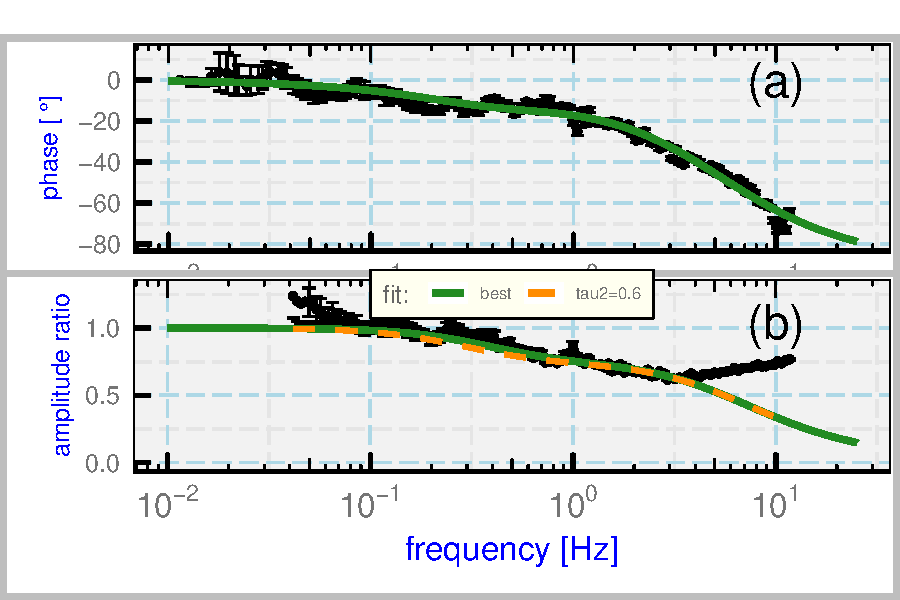
\includegraphics[width=12cm]{figure/fig2} \end{center}

\caption[Phase and amplitude ratio (or gain) for the measured recovery temperature
relative to dynamic heating.]{(a): The ratio of the spectral amplitude for the measurement
of recovery temperature ($T_{m}(t)$) to that for dynamic heating
($Q$), shown as the plotted data points. There are additional data
points at frequencies below about 0.04 Hz that do not appear in this
plot because they lie above the upper limit for the ordinate. The
green line is the prediction from the transfer function determined
from the best-fit values matching the phase lag between these variables,
and the dashed orange line is a similar result with the second time
constant $\tau_{2}$ increased from 0.447 to \unit{0.6\,s} to illustrate
sensitivity to this parameter.\protect \\
(b): Phase of measured recovery temperature relative to dynamic
heating, for the measurements (with error bars) and for the theoretical
response for the best-fit parameters (green line). The error bars
indicate two-standard-deviation ranges in the mean at each plotted
point. Data for both plots are from the  flight segments listed in Table\ 1.
{\label{fig:Vphase}}}
\end{figure}

The ratio of the amplitude of the response to that of the
dynamic-heating signal, used as an estimate of the gain of the transfer
function, is shown in Fig.~\ref{fig:Vphase}a. It is useful to consider
both the amplitude and phase when determining the response parameters
because, as shown in Fig.~\ref{fig:LTsolution}, the amplitude of the
transfer function is more sensitive to \(\tau_{2}\) than the phase but
\(\tau_{1}\) is a very sensitive predictor of the phase at high
frequency. For the set of favored parameters, Fig.~\ref{fig:Vphase}a
shows the standard prediction and another with \(\tau_{2}\) set to
\unit{0.6\,s} instead, to show the sensitivity of this result to that
parameter. The best prediction based on the measured phases consistently
underestimates the ratio of spectra for frequencies below about
\unit{0.1\,Hz} and above about \unit{3\,Hz} but is reasonably consistent
with the observed ratio between those limits. Below \unit{0.1\,Hz}
variance spectra indicate that the sensor is responding to real
fluctuations in temperature not attributable to dynamic heating, as
would be expected at these low frequencies. Above \unit{3\,Hz} the
prediction is much too low. This could arise because there is spurious
variance in the measurement \(T_m(t)\) not caused by dynamic heating or
because the measurement of dynamic heating is attenuated at high
frequency. The variance spectra (not shown) suggest both may contribute
to the discrepancy, but excess variance in the measured recovery
temperature appears to be the more significant problem. The variance
spectrum of \(T_m(t)\) is reduced substantially above \unit{3\,Hz} if it
is multiplied by the squared coherency between \(T_m(t)\) and \(Q\), so
most of the excess variance above this frequency is apparently not
attributable to fluctuations in dynamic heating. Exclusion of these
measurements from the fit is therefore reasonable.

The fit procedure used Eq.~\eqref{eq:responseAmp} and
Eq.~\eqref{eq:responsePhase} to find the theoretical value of the
amplitude ratio and phase at each frequency represented in the
observations. For assumed values of the three parameters \(a\),
\(\tau_{1}\) and \(\tau_{2}\), a chi-square was calculated from the
differences between these theoretical values and the observed values.
The frequencies used for the fit were 0.01 to \unit{12\,Hz} for the
measurements of phase and 0.1 to \unit{3\,Hz} for the measurements of
amplitude ratio, to avoid regions where effects other than dynamic
heating appear to bias the measurements. Then a search procedure varied
these parameters to seek the minimum value of the chi-square. The
resulting values were \(a\)= 0.7, \(\tau_{1}\)= 0.031 and \(\tau_{2}\)=
0.56. The chi-square for the fit is about 18 times larger than expected
if the fit represents the measurements to measurement uncertainty, so it
is difficult to assign uncertainty limits to this result on the basis of
this fit because of this not-understood excess chi-square, but the fit
minimum distinguished nearby values to about three significant digits in
all three parameters. The Hessian from the fit implies that the results
with standard uncertainties are \(a\)= 0.703 \(\pm\) 0.003,
\(\tau_{1}\)=0.031\(\pm\)\ensuremath{3\times 10^{-4}}\unit{\,s} and
\(\tau_{2}\)=0.56 \(\pm\) 0.02\unit{\,s}.

To complete the iteration discussed earlier, the measured recovery
temperature was then corrected as described in Appendix~A, using the
parameters from this first fit to predict the actual recovery
temperature \(T_{r}(t)\). The calculation of phase and amplitude was
repeated After recalculating \(Q\) using Eq.~\eqref{eq:DHterm} and that
prediction of \(T_{r}(t)\), the results were fitted again by adjusting
the fit parameters. Only insignificant changes, much smaller than the
quoted uncertainties, resulted from this iteration.

\subsubsection{\texorpdfstring{Heated
sensors\label{subsec:Heated-sensors}}{Heated sensors}}

Measurements from two slower sensors, a heated Goodrich/Rosemount 102
sensor and a similar Harco Model 100009-1 Deiced TAT sensor, have also
been evaluated, but only the latter (hereafter called the ``heated
sensor'') is discussed here because they have similar response. The
spectral variance for both these measurements has apparent rapid
attenuation beginning at about \unit{0.1\,Hz}, as shown in
Fig.~\ref{fig:HARCOSpec}, and the response is attenuated seriously above
about \unit{1\,Hz}. To find the transfer function for this sensor,
boundary-layer flight segments from the SOCRATES and CSET projects were
compiled into one data set from the flight periods shown in Table~2.

Fits using the three-parameter representation of the transfer function
were unsatisfactory for the heated sensor, apparently because
fluctuations caused by dynamic heating were not as dominating a cause of
the temperature fluctuations as they were in the measurements used for
the unheated sensor. Therefore a different approach was used here.
Because the evaluation in Sect.~\ref{subsec:The-unheated-Rosemount}
provides a good representation of the unheated sensor, the measurements
from that sensor, corrected as described in Appendix~A, were used as the
reference for the assumed-correct recovery temperature. Then the phase
and amplitude ratio were found for the transfer function required to
produce the heated-probe measurements from the unheated-probe
measurements. This did not require any assumptions about equations or
parameters determining the transfer function for the heated sensor.

\begin{figure}

\begin{center}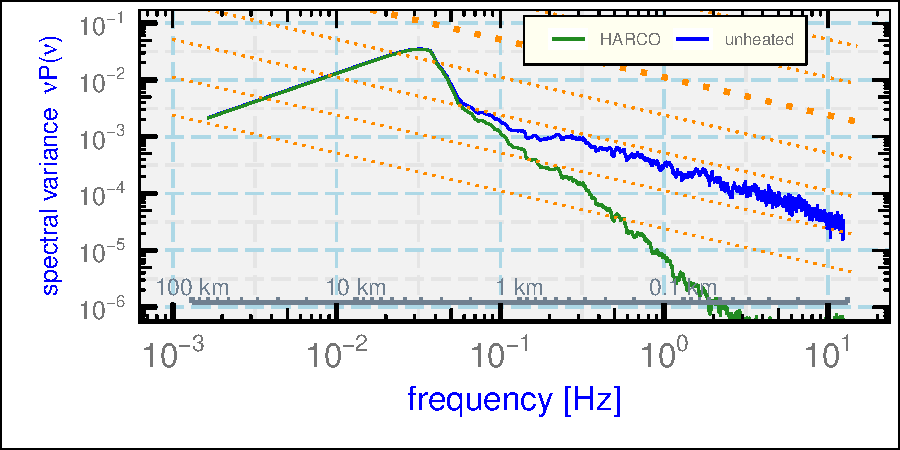
\includegraphics[width=8.3cm,height=5cm]{figure/fig3} \end{center}
\caption{Spectral variance $P(\nu)$ weighted by frequency ($\nu$) for the recovery temperature measured by a heated and an unheated temperature sensor. The background includes orange dotted lines denoting $-2/3$ slope and the wavelength scale is determined from the average airspeed.\label{fig:HARCOSpec}}
\end{figure}

\begin{table}[t]
%\begin{centering}
\caption{Flight segments used to determine the response characteristics of
a heated sensor.}
\begin{tabular}{|c|c|c|}
\hline 
\bf{Project / Flight} & \bf{start [UTC]} & \bf{end [UTC}\tabularnewline
\hline 
\hline 
CSET / 5 & 2015-07-14 17:52:00 & 18:02:00\tabularnewline
\hline 
CSET / 5 & 2015-07-14 19:45:30 & 19:55:30\tabularnewline
\hline 
CSET / 5 & 2015-07-14 20:37:17 & 20:47:17\tabularnewline
\hline 
SOCRATES / 15 & 2018-02-24 5:52:00 & 6:02:00\tabularnewline
\hline 
SOCRATES / 15 & 2018-02-24 6:05:00 & 6:15:00\tabularnewline
\hline 
\end{tabular}
%\par\end{centering}
\end{table}

\begin{figure}

\begin{center}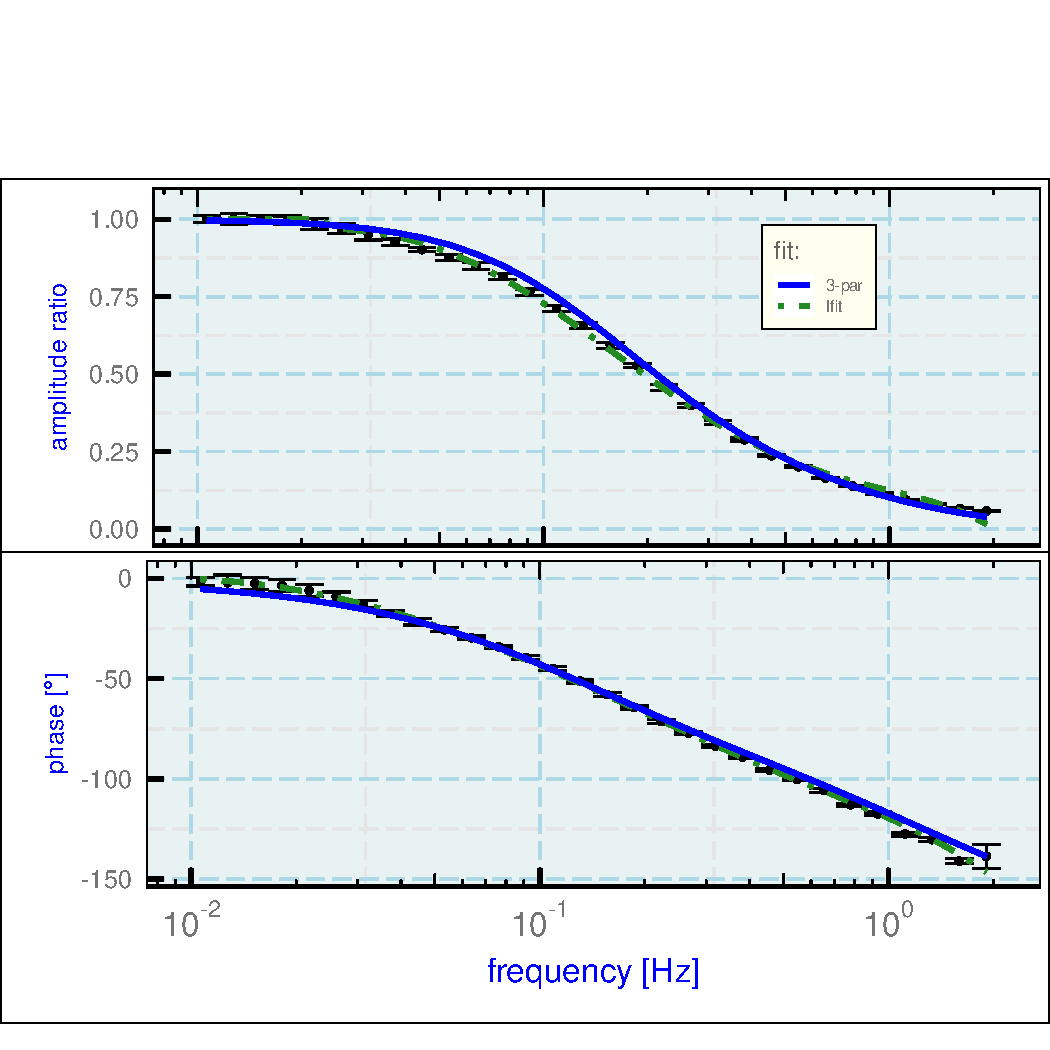
\includegraphics[width=12cm]{figure/fig4} \end{center}

\caption[The amplitude ratio and phase for the transfer function characterizing a heated temperature sensor. ]{The amplitude ratio (top) and phase (bottom) for the transfer function characterizing
a heated temperature sensor. The measurements are indicated
by error bars that show two-standard-deviation limits from the mean
value). Two fits to the measurements, one based on the three-parameter
representation ("3-par") and one on a polynomial fit ("lfit"),
are described in the text.{\label{fig:GVHARCO}}}
\end{figure}

The measured phase and amplitude ratio for this data set are shown in
Fig.~\ref{fig:GVHARCO}. The fits for the response function defined by
Eq.~\eqref{eq:responseAmp} and Eq.~\eqref{eq:responsePhase} are shown as
the blue lines labelled ``3-par'' in that figure. The fitted values for
\{\(a,\,\tau_{1},\,\tau_{2}\)\} were \{0, 0.108\unit{\,s},
1.28\unit{\,s}\}, and to obtain this result the fit had to be
constrained to keep \(a\) non-negative. A value of zero for the
parameter \(a\) would indicate that no heat is transferred from the
sensing wire to the air, but instead all is transferred to the support
which has a relatively slow characteristic response.

The three-parameter fit is not consistent with the measurement errors
even though it provides an approximate representation of the transfer
function. The apparent reason is that there is conflict between the
constraints imposed by the amplitude ratio and the phase, such that
either could be represented reasonably but not both. Because the
three-parameter fit distorted the measured result, fits in the logarithm
of the frequency were used to provide a better representation of the
measurements, as shown by the dashed green lines labelled ``lfit''.
Those fits are given by these equations and coefficients, with
\(x=\log_{e}(\nu/\nu_{0})\) where \(\nu\) is the frequency,
\(\omega=2\pi\nu\) and \(\nu_{0}\)=\unit{1\,Hz}: \begin{align}
\hskip1em\mathrm{for}\ \nu>0.024\,\mathrm{Hz},\quad H(\omega)= & (h_{0}+h_{1}x+h_{2}x^{3}+h_{3}x^{4}+h_{4}x^{5})e^{i\phi(\omega)}{\label{eq:lfitH}} \\
\hskip1em\mathrm{for}\ \nu\leq0.024\,\mathrm{Hz},\quad H(\omega)= & e^{i\phi(\omega)} \\
\hskip1em\mathrm{for}\ \mathrm{all}\ \nu,\quad\phi(\omega)= & p_{0}+p_{1}x+p_{2}x^{2}+p_{3}\arctan(\nu/\nu_{0})
\end{align} The coefficients obtained by fitting to the observations are
\(h_{0-4}\)=\{\(0.124\), \(-0.116\), \(-0.0929\), \(-0.0374\),
\(-0.00391\)\} and \(p_{0-3}\)= \{\(-190.3\), \(-78.7\), \(-8.16\),
\(90.3\)\}. This fit (with negative-frequency values defined as the
complex conjugate of the values at the corresponding positive frequency)
represents the transfer function better than the three-parameter fit,
although the fit is not valid above about \unit{2\,Hz} because those
values were not constrained by the measurements.

\subsubsection{\texorpdfstring{Expected dependence on flight
conditions\label{subsec:Expected-dependence-on}}{Expected dependence on flight conditions}}

Based on measurements in a wind tunnel, \citet{GoodrichTR5755} indicated
that the fast-response characteristic time \(\tau_{1}\) for the unheated
sensor varies approximately as \(\log(Z^{-0.68})\) where
\(Z=M\rho_{a}/\rho_{s}\) with \(M\) the Mach number, \(\rho_{a}\) the
air density and \(\rho_{s}\) the air density under standard conditions.
The mean value of \(Z\) for the flight segments used to find the
best-fit parameters for the unheated sensor on the C-130 was \(Z=0.3\),
so this suggests that the first characteristic time for that sensor is
best represented by \begin{equation}
\tau_{1}^{\prime}(Z)=\tau_{1}\left(\frac{0.3}{Z}\right)^{0.68}\,\,\,.{\label{eq:tau1prime}}
\end{equation} For a flight segment at about \unit{11.5\,km} altitude,
where the mean value of \(Z\) was 0.228, \(\tau_1\) was found to be
\unit{0.037\,s}, exactly matching the prediction of
\eqref{eq:tau1prime}, so this provides some limited support for that
equation. For these reasons, the values of \(\tau_1\) found in preceding
sections have been adjusted to a reference value of \(Z=0.3\) in
Table~\ref{tab:Parameters}. For other conditions, it is suggested that
the best estimate will be to multiply \(\tau_{1}\) by
\((0.3/Z)^{0.68}\).

\begin{table}[t]
\caption{Parameters for the time response of available temperature sensors
on the NSF/NCAR aircraft, adjusted to $Z=0.3$. For other conditions,
scale as represented for $\tau_{1}^{\prime}$ in 
Eq.\ \eqref{eq:tau1prime}. Parameters for the unheated sensor were also determined for measurements on the GV, with the result {0.73, 0.035, 0.36},
but the fit was less satisfactory than the one for the C-130 
so the fit in the table has been used in this paper for measurements from both aircraft.{\label{tab:Parameters}}}
\begin{tabular}{|c|c|c|c|}
\hline 
\bf{sensor} & $a$ & $\tau_{1}$ [s] & $\tau_{2}$ [s]\tabularnewline
\hline 
\hline 
"unheated" (Rosemount 102E4AL) & 0.73 & 0.031 & 0.45\tabularnewline
\hline 
"heated" (HARCO Model 100009-1 Deiced TAT)& 0.0 & 0.13 & 1.28\tabularnewline
\hline 
\end{tabular}
\end{table}

\section{\texorpdfstring{Correcting for Dynamic
Heating\label{sec:Correcting-for-Dynamic}}{Correcting for Dynamic Heating}}

In conventional processing to calculate the ambient air temperature, an
independently determined estimate of dynamic heating is subtracted from
the measured temperature, as described in
Sect.~\ref{subsec:Dynamic-heating}. When the sensor cannot respond to
the measured fluctuations in dynamic heating, this procedure introduces
errors and excess noise into the resulting air temperature. Data
processing should instead apply a correction that represents how dynamic
heating affects the measurement from the sensor, not how it affects the
recovery temperature.

Figure~\ref{fig:f5} illustrates the problem. The measurements are from a
low-level flight segment over the ocean where other indications are
reasonably consistent with an inertial subrange. The heated sensor gives
the measurement conventionally assumed to be the recovery temperature,
as shown by the dashed blue line. The slow sensor does not respond to
the high-frequency changes in dynamic heating, and as a result
subtraction of the dynamic-heating term to obtain the air temperature
(shown as the thick red line) introduces erroneous high-frequency
fluctuations in the result that are opposite to the fluctuations in
dynamic heating. These fluctuations are not real; they occur because the
sensor does not respond to the fluctuations in dynamic heating so
subtraction of those fluctuations introduces erroneous fluctuations in
the calculated air temperature. A similar plot for the unheated sensor
indicates a similar effect, although it is reduced in magnitude because
that sensor has much faster response.

\begin{figure}

\begin{center}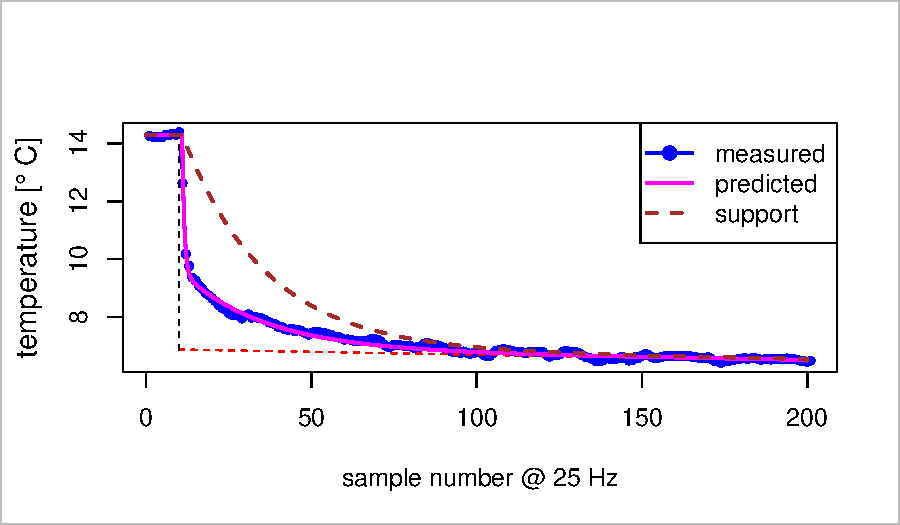
\includegraphics[width=8.3cm]{figure/fig5} \end{center}
\caption{The measured recovery temperature ($T_m$) from an unheated sensor, the dynamic heating ($Q$), and the result of using Eqs.\ \eqref{eq:DHterm} and \eqref{eq:recoveryTemperature} to calculate the air temperature ($T_a$). Mean values have been subtracted from these variables to facilitate comparison. Data from VOCALS flight 3.\label{fig:f5}}
\end{figure}

The new approach followed here is to filter the dynamic-heating term so
that only the actual sensor response to dynamic heating is subtracted
from the measurement. This is made possible by the assumed linearity in
response of the sensor, which is required if this part of the response
is to be separated from the more general response to the combination of
dynamic heating and true fluctuations in temperature. The proposed
filtering removes a significant source of erroneous fluctuations present
in many temperature measurements made from research aircraft.

The filtered response has been obtained from the transfer function in
three ways, by integration of the differential equations
(Eqs.~\eqref{eq:Ts} and \eqref{eq:Tm}) applied to \(Q\), by Fourier
transforms using the transfer function, and by applying a digital filter
designed from the transfer function. The digital filter was designed
using standard methods as outlined in, e.g.,
\citet{Press:1992:NRC:148286}; details and the coefficients used are
available in the Workflow document that accompanies this paper. All
three methods produce almost equivalent results. The filtered
dynamic-heating adjustment will be denoted \(Q^{\prime}\), and the
calculated air temperature \(T_a^\prime\) then becomes \begin{equation}
T^{\prime}_{a}(t)=T_{m}(t)-Q^{\prime}(t){\label{eq:QprimeCorr}}
\end{equation} instead of Eq.~\eqref{eq:recoveryTemperature}.

\begin{figure}

\begin{center}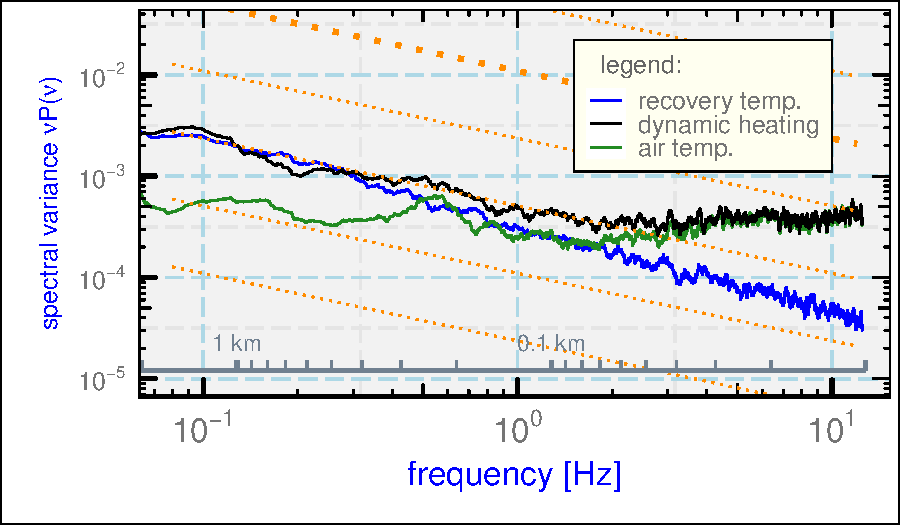
\includegraphics[width=12cm,height=5cm]{figure/fig6} \end{center}

\caption[For an unheated sensor, variance spectra for the
dynamic-heating term after application of three different filters.
Also, variance spectra for the measurement of recovery temperature
and ambient temperature calculated using the filtered dynamic-heating
term. ]{Variance spectra for an unheated sensor, for a boundary-layer
flight segment from SOCRATES flight 15, 6:02:00 to 6:13:00 UTC.
The backgrounds include orange dotted lines denoting $-2/3$ slope,
and the wavelength scale is determined from the average airspeed.\protect \\
(a): The dynamic-heating term ("Q") and the filtered term
obtained by integrating the differential equations for the derivatives
("DiffEq"), by Fourier transformation with application of the
transfer function ("FFT"), or applying the digital filter ("filter").
The result for the latter is so close to that for "FFT" that it
is obscured in this plot.\protect \\ 
(b): The measurement of recovery temperature and ambient temperature
calculated using the digitally filtered dynamic-heating term. The original
variable for ambient temperature based on standard processing 
("with std Q") is also shown.{\label{fig:Integration}}}

\end{figure}

Figure~\ref{fig:Integration}a shows the variance spectra that result
from all three methods when applied to measurements from an unheated
sensor. The measured dynamic-heating term (\(Q\)) in this case has
substantial high-frequency variance in excess of expectations for an
inertial subrange. Lenschow (in \citet{cooper2016ncartn}) argued that
this is the result of resonance in the sampling lines, so it does not
reflect a true influence on the recovery temperature. The modified
variance spectrum obtained by integration of the underlying differential
equations is shown as the orange line labelled ``DiffEq''. The
dynamic-heating correction is appropriately attenuated at high frequency
after this integration. The results obtained after application of a
digital filter representing the transfer function, labelled ``filter'',
or after Fourier transformation, labelled ``FFT'', are mostly
overlapping. These latter corrected estimates of the dynamic heating are
attenuated even more than the result from numerical integration and are
in better agreement with the predicted effect of the transfer function,
which for example predicts attenuation of the variance spectrum by a
factor of 0.096 for the component with frequency \unit{10\,Hz}. The
numerical integration was closer to the results of the filter after the
measurements were interpolated to \unit{125\,Hz} with \unit{25\,Hz}
smoothing, integrated, and then resampled to obtain \unit{25\,Hz}
measurements, so the high-frequency discrepancy appears to result from
accumulating numerical errors in the integration. The equivalence of the
results from the digital filter and from Fourier transformation with
application of the transfer function supports the validity of these
results and suggests that these are preferable and equivalent methods
for filtering dynamic heating to match the response of the temperature
sensor.

A revised estimate of the ambient air temperature was then calculated
using Eq.~\eqref{eq:QprimeCorr} and the corrected dynamic-heating term
\(Q^{\prime}\). The spectral variance for this air temperature, shown in
Fig.~\ref{fig:Integration}b as the blue line, is improved considerably
at high frequency vs.~that using the standard correction. Even at
\unit{1\,Hz}, filtering the dynamic-heating term removes a significant
and erroneous contribution to the variance in the measured air
temperature.

In the case of the heated sensors, the revision is still more
significant because they respond more slowly. Figure~\ref{fig:HarcoQ}a
shows the result of filtering the dynamic-heating term for a heated
sensor. The result of integration (``DiffEq'') and the digital filter
(``filter'') are almost identical so there is no evidence of the
numerical problems that were encountered with the integration for the
unheated sensor. The difference vs.~the original is quite dramatic even
at \unit{1\,Hz}, and the errors are significant for all frequencies
above about \unit{0.1\,Hz}.

\begin{figure}

\begin{center}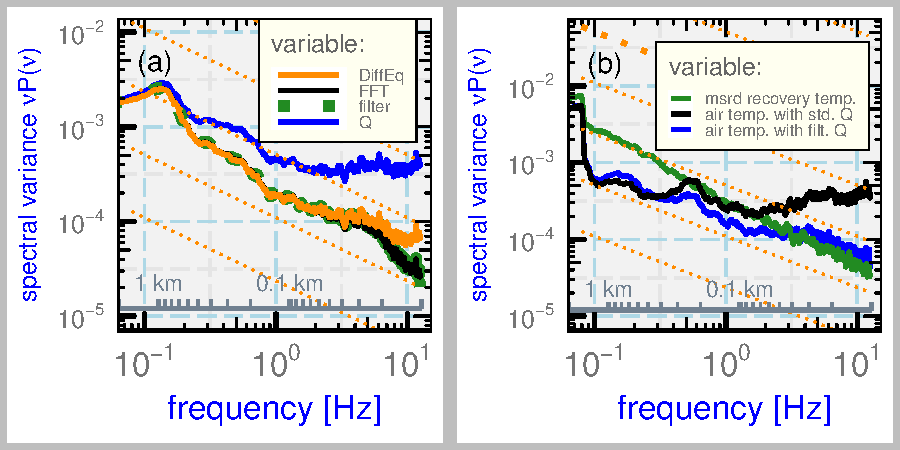
\includegraphics[width=12cm,height=5cm]{figure/fig7} \end{center}

\caption[Variance spectra for the heated temperature sensor: The unmodified dynamic-heating
term and two filtered terms. Also, the air temperature as modified
by filtering the dynamic-heating term.]{Variance spectra for a heated temperature sensor. (Data from
the WECAN project, flight 17, 18:04:00 to 18:35:00 UTC.) 
The backgrounds include orange dotted lines denoting $-2/3$ slope and the wavelength scale is determined from the average airspeed.\protect \\
(a): The unmodified dynamic-heating term ("Q") and the two
corrected terms. The results from solving the differential equations
("DiffEq") or from application of the digital filter ("filter")
are overlapping and indistinguishable in this figure.\protect \\
(b): The air temperature as modified by filtering the dynamic-heating
term (blue line). The other plotted spectra are for the measured recovery
temperature and the air temperature with the conventional dynamic-heating
correction.{\label{fig:HarcoQ}}}
\end{figure}

Figure~\ref{fig:HarcoQ}b shows how this affects the spectral variance of
the measured air temperature. The slow response of this sensor causes
the measured recovery temperature (green line) to have very low spectral
variance when the frequency is above \unit{1\,Hz}, so the variance in
the standard air-temperature measurement in this frequency range is
almost entirely caused by erroneous adjustment for fluctuations in
dynamic heating to which the sensor does not respond. The correction
procedure using a filtered dynamic-heating correction removes this
excess spectral variance and produces a signal where the variance for
frequencies above about \unit{0.1\,Hz} arises primarily from variance in
the measured recovery temperature. The variance spectrum for the
conventionally processed temperature looks approximately as might be
expected in an inertial subrange, but the variance above about
\unit{0.5\,Hz} is a false signal that does not arise from real variance
in temperature. It therefore becomes very important to use this revised
processing scheme to avoid erroneous measurements even for changes
occurring over \unit{5\,s} or more. Because the corrected variance
spectra properly represent how the temperature sensor responds to
dynamic-heating fluctuations, filtering \(Q\) removes substantial
erroneous variability otherwise present in the calculated air
temperature.

\begin{figure}

\begin{center}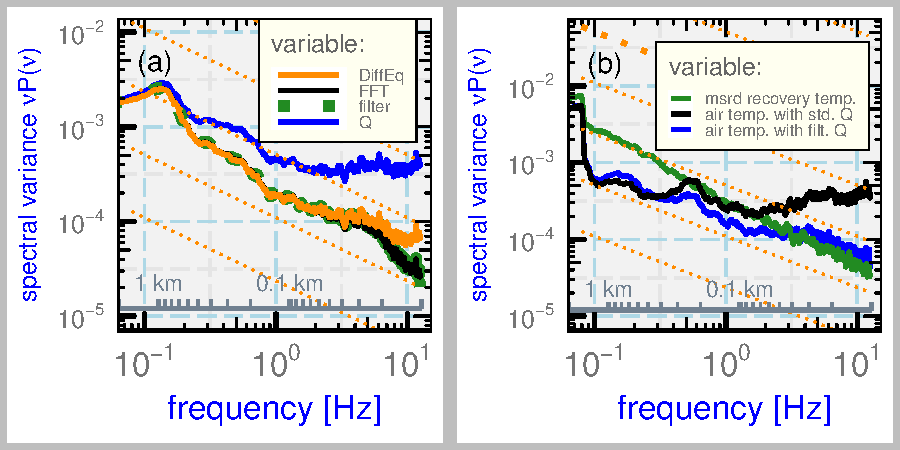
\includegraphics[width=12cm,height=5cm]{figure/fig8} \end{center}

\caption[Comparison of the original calculated air temperature and the same temperature
after filtering the dynamic-heating correction, for an unheated sensor and a heated sensor. ]{Comparison of the original calculated air temperature and the same temperature
after filtering the dynamic-heating correction:\protect \\
(a): An unheated sensor, VOCALS project, flight 3, time after 8:01:00 UTC; (b): A heated sensor, WECAN project, flight 17. time after 18:13:00 UTC. {\label{fig:ATATF}}}
\end{figure}

Fig.~\ref{fig:ATATF}a illustrates the removal of erroneous structure by
filtering for the unheated sensor, and Fig.~\ref{fig:ATATF}b shows a
similar example for the heated sensor. These figures illustrate that the
erroneous fluctuations in the standard measurements can be important in
many potential uses of these measurements and should be removed as part
of standard processing. The effect is particularly significant for the
heated sensor, for which the conventionally processed temperature has
large fluctuations that are caused by subtraction of fluctuations in
dynamic heating to which the sensor does not respond. These do not arise
from real fluctuations in ambient air temperature.

\section{\texorpdfstring{The Flux Density of Sensible
Heat\label{sec:flux-density}}{The Flux Density of Sensible Heat}}

\subsection{\texorpdfstring{Outline of the correction
procedure\label{subsec:Outline-correction}}{Outline of the correction procedure}}

Most past studies of temperature-sensor response (e.g.,
\citet{mccarthy1973method}, \citet{nicholls1978measurements},
\citet{InverarityJTech2000}) applied corrections to the air temperature
after compensation for dynamic heating. That applies the full correction
for dynamic heating \(Q\) without considering that the sensor may
respond only partly to high-frequency fluctuations in \(Q\), which was
shown in Sect.~\ref{sec:Correcting-for-Dynamic} to lead to erroneous
noise in the air temperature. Then that noise is amplified by the
correction procedure. These errors are avoided if corrections for time
response are applied instead to the measurement of the recovery
temperature. The amplification of signals by application of the transfer
function restores the fluctuations produced by dynamic heating, and
those fluctuations are then removed by subtracting the measured
(unfiltered) dynamic heating term from the corrected recovery
temperature.

The eddy-correlation calculation used here starts with the Fourier
representation of the measured recovery temperature. (Fourier transforms
are denoted here by the symbol ``~\(\widehat{~}\)~'' over variables.)
The measurement is related to the true recovery temperature via
\(\hat{T}_{m}(\nu)=H(\nu)\hat{T}_{r}(\nu)\) where \(H(\nu)\) is the
frequency-domain transfer function. The true recovery temperature will
be the inverse Fourier transform of
\(\hat{T}_{r}(\nu)=\hat{T}_{m}(\nu)/H(\nu)\). The Fourier representation
of the air temperature is then
\(\hat{T}_{a}(\nu)=\hat{T}_{m}(\nu)/H(\nu)-\hat{Q}(\nu)\), which
includes both the correction for time response and the subtraction of
dynamic heating. Multiplication by the complex conjugate of the Fourier
representation of the updraft gives the cospectrum representing the flux
of sensible heat, with an appropriate scale factor as specified in
Eq.~\eqref{eq:heatFlux}. The resulting cospectrum is then integrated
over an appropriate wavelength range to produce the measured flux
density of sensible heat. This will normally exclude wavelengths greater
than a few kilometers so that the estimate represents the turbulent
contribution.

\subsection{Examples of Measured Cospectra and Fluxes}

Two examples of measured cospectra illustrate the effect of the
correction. The first example is from the SOCRATES project, 24 January
2018, 6:00:00 to 6:15:00~UTC, and the second is from the CSET project, 1
August 2015, from various segments from 16:00:00 to 19:15:00~UTC. The
flight segments were all at low level (\unit{150\,m}) in the marine
boundary layer over the Pacific Ocean. An unheated sensor was used to
measure temperature on these flights. In each case, the cospectra from
three flight segments of \unit{5\,min} (SOCRATES) or \unit{10\,min}
(CSET) duration were averaged to produce the measured cospectra.
Uncertainties in this measurement and common features of the atmospheric
boundary layer are discussed by \citet{lenschow95micro}.
\citet{lenschow1986length} suggested that, for 10\% uncertainty in a
measurement of scalar flux, an averaging distance of 100--500 times the
boundary-layer height is required. (See also \citet{lenschow1994long}.)
The flight segments in these two cases span about 80--150 times the
boundary-layer height, so they are marginal by this criterion, but the
measurements still serve to illustrate the effect of the proposed
correction.

\begin{figure}

\begin{center}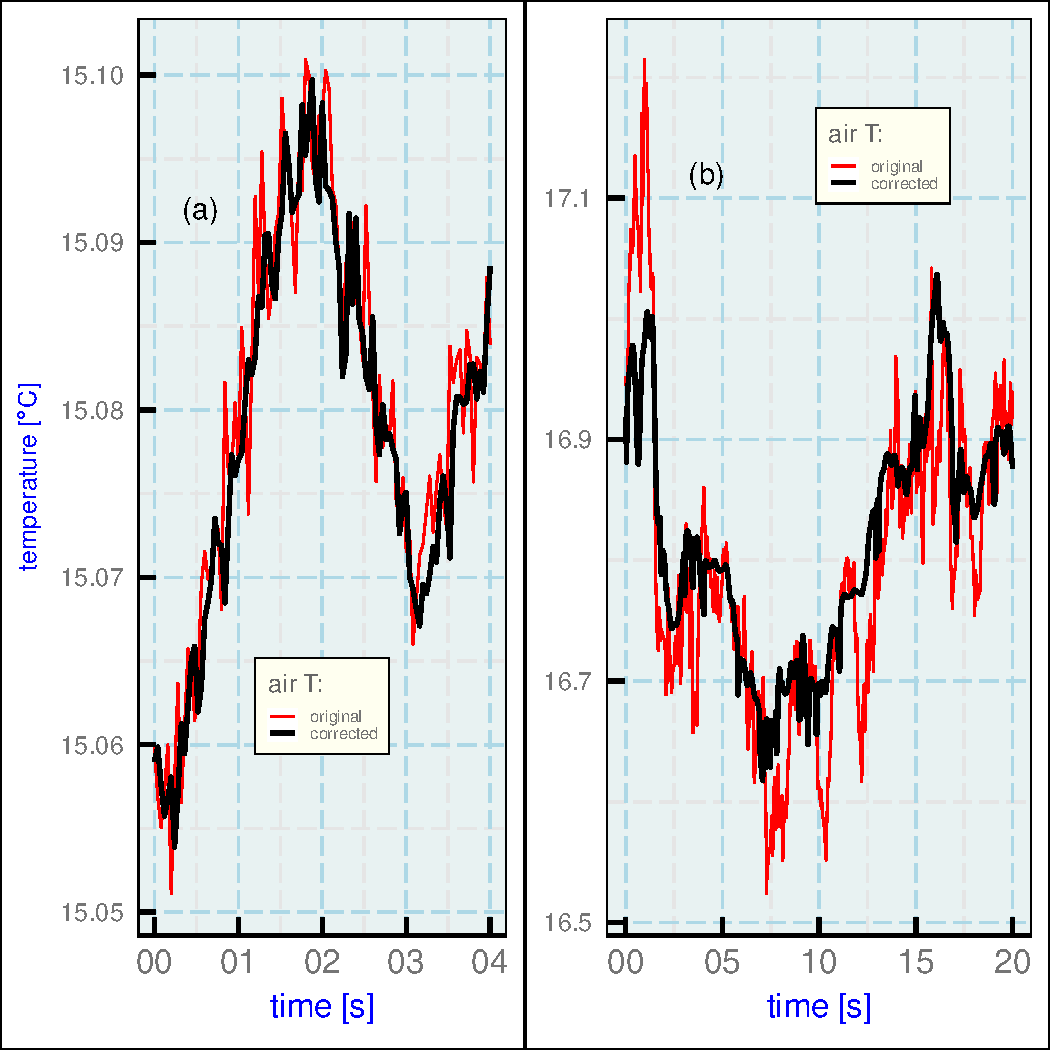
\includegraphics[width=12cm]{figure/fig9} \end{center}

\caption{The corrected flux of sensible heat, weighted by the frequency $\nu$,
for low-level flight segments over the Pacific Ocean. The "exceedance"
is the complement of the cumulative distribution function (i.e., the
sum of contributions from frequencies above the plotted value), and
the dashed exceedance line is that without transfer-function
correction but with adjustment of the dynamic-heating term to incorporate
the estimated response of the temperature sensor. For the SOCRATES example,
the total flux is \unit{23.6\,W\,m^{-2}} and the flux contributed from wavelengths smaller than \unit{2\,km} is \unit{23.5\,W\,m^{-1}}, while the corresponding numbers for the CSET example are 16.0 and \unit{15.4\,W\,m^{-2}}. The dashed black
line shows the frequency limit that corresponds to a wavelength of
\unit{2\,km}.{\label{fig:SOCp1}}}
\end{figure}

The corrected cospectra are shown in Fig.~\ref{fig:SOCp1}. This plot
format is unconventional so some explanation is provided here. The
cospectrum can be positive or negative, so it is usually plotted using a
linear ordinate scale. However, the range of ordinate values is
displayed better with a logarithmic scale, even after weighting the
cospectrum by frequency. The compromise made in this plot is to use a
logarithmic scale but plot negative values with sign reversed and with a
different color, here red instead of blue. Other features of this plot
and computation conventions include the following:

\begin{enumerate}
\def\labelenumi{\arabic{enumi}.}
\item
  The cospectra have been smoothed using width-3 moving averages for
  frequencies above \unit{0.01\,Hz}, then width-5 for frequencies above
  \unit{0.1\,Hz}, then width-17 for frequencies above \unit{1\,Hz}. For
  these \unit{5\,min} flight legs and for \unit{25\,Hz} measurements,
  the maximum smoothing interval is about \unit{0.05\,Hz} so most
  spectral features are retained even with this strong smoothing.
  Additional smoothing results from averaging three cospectra to obtain
  the plotted values.
\item
  Further smoothing is included by binning the results into 100
  logarithmically spaced intervals in frequency and averaging in those
  bins. That results in the blue dots (or dark red dots for negative
  points).
\item
  The listed ``total'' flux is that arising from the part of the flux
  with frequency above \unit{0.01\,Hz}. This frequency limit restricts
  the calculation to wavelengths smaller than about \unit{13\,km}.
  Another measurement of the flux is calculated for wavelengths below
  \unit{2\,km}. That or a still smaller wavelength limit is a reasonable
  measure of the part of the flux contributed by turbulent air motions
  in the boundary layer, so that second measurement is used as the
  primary measurement in this study.
\item
  The grey line labelled ``exceedance'' is a cumulative distribution
  function for the cospectrum, called ``exceedance'' because it is the
  contribution from all frequencies \emph{higher} than the indicated
  value. (This has been called the ``ogive'' by, e.g.,
  \citet{Foken2006ACPclosure}.) At high frequency on a logarithmic
  scale, where some of the most interesting variation is located, the
  exceedance distribution is more informative that the conventional
  cumulative distribution. Its units are \unit{W\,m^{-2}}, not
  \unit{W\,m^{-2}} per logarithmic interval as is the case for the
  weighted cospectrum.
\end{enumerate}

The exceedance distributions before correction, shown as the dashed grey
lines, were calculated using dynamic-heating terms filtered to match the
responses of the sensors, but otherwise were not corrected. About 33\%
of the flux contributed by wavelengths smaller than \unit{2\,km} would
be missed without correction for time response as represented by the
transfer function, as shown by the solid grey lines. The underestimation
is particularly serious at higher frequencies: In both cases the
measured contribution from frequencies above \unit{1\,Hz} is more than
twice as large after correction as it is without correction. A
significant contribution to the error is the phase shift that causes the
measured temperature to be shifted in phase relative to the updraft, as
shown in Fig.~1.

\citet{LawsonRodi1992} estimated that, in comparison to their fast
thermocouple sensor, the unheated Rosemount sensor underestimated the
flux by about 21\%. The magnitude of the correction here is larger than
their estimated error, but the flight speed of the aircraft was about
30\% greater than that of the aircraft they used so a larger error would
be expected.

Because the corrected cospectrum appears realistic at frequencies of
\unit{1\,Hz} and above, it is possible to judge if the frequency
coverage is adequate. In this case, the exceedance curve is less than
2\% at \unit{10\,Hz} and falls rapidly above that frequency, even after
correction, so it appears likely that additional contributions from
higher frequencies can go unmeasured without introducing serious errors
into the measurement of flux. Additional guidance regarding the expected
shape of the cospectrum and the required frequency response is provided
by \citet{lenschow95micro}. The generalized cospectra provided there
suggest that, for flight at \unit{130\,m\,s^{-1}}, frequencies up to
about \unit{1.3\,Hz}--\unit{10\,Hz}, depending on altitude, must be
measured. The higher frequency limit applies to low-level flight at
about \unit{30\,m} above the surface. Those results suggest that, if the
measurements are corrected as suggested here, reliable measurements of
sensible-heat flux can be made with the unheated sensor.

\subsection{Evidence from Simulated Measurements}

As a test of the approach described in the preceding section, a
simulated case was analyzed in the same way. Time series were generated
representing isotropic wind measurements by starting with a
Gaussian-noise spectrum, weighting the Fourier components to obtain a
\(-5/3\) slope, and then using an inverse Fourier transform to
reconstruct the simulated measurement series.

A time series for temperature was generated similarly but scaled by a
factor of \unit{0.2^{\circ}C\,m^{-1}\,s}, and then a correlation of 0.3
was introduced between temperature and updraft fluctuations. In this
simulation, about 15\% of the flux from wavelengths below \unit{2.5\,km}
is contributed by frequencies above \unit{1\,Hz}, where the sensor may
respond incompletely to the fluctuations and underestimate the flux.

\begin{figure}

\begin{center}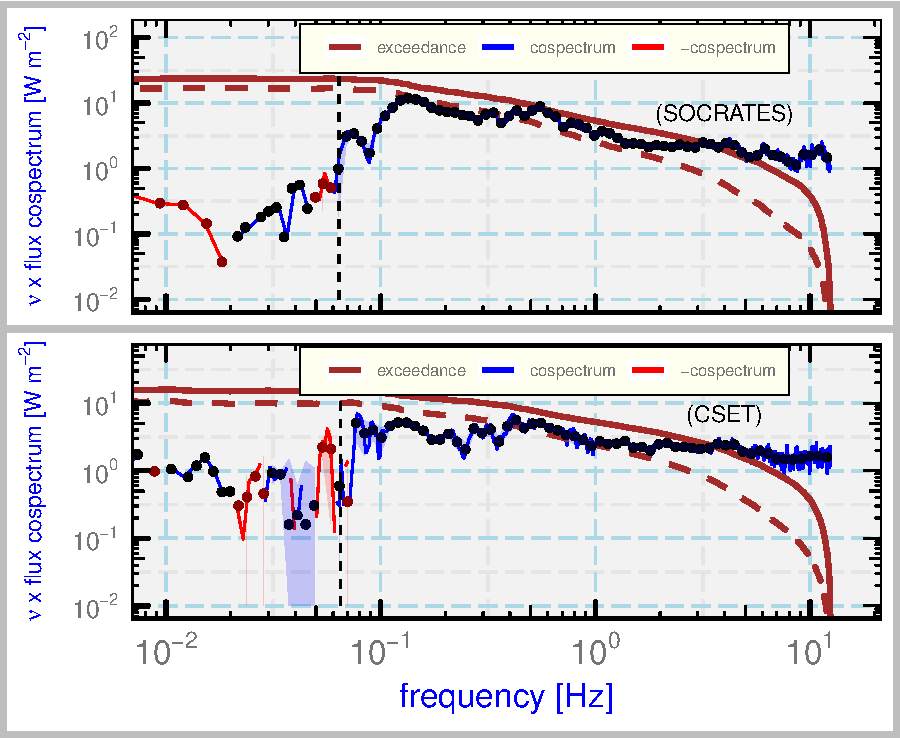
\includegraphics[width=8.3cm,height=5cm]{figure/fig10} \end{center}
\caption{The cospectrum for the flux of sensible heat (blue line), weighted by frequency $\nu$, for the simulated data generated as described in the text. Three \unit{10\,min} segments of simulated \unit{25\,Hz} data were averaged. The measured cospectrum was obtained by filtering the simulated recovery temperature and subtracting the correction for dynamic heating. For the generated and measured cospectra, filled circles indicate the average values calculated in 50 logarithmically spaced intervals, and for the measured cospectrum shading indicates the standard deviation in those intervals. The exceedance lines show the contribution to flux from frequencies higher than the plotted frequency. The corrected cospectrum is not shown but is consistent with the generated cospectrum, as demonstrated by the agreement between the generated exceedance and the corrected exceedance. The units for the exceedance distributions are \unit{W\,m^{-2}}, while the units for the weighted flux cospectra are \unit{W\,m^{-2}} per unit logarithmic increment. The frequency corresponding to a wavelength of \unit{2.5\,km} is denoted by the heavy dashed-black line.\label{fig:simF}}
\end{figure}

Figure~\ref{fig:simF} shows (as the green line) how the simulated
cospectrum would be measured by a sensor with response parameters
\{\(a,\,\tau_{1},\,\tau_{2}\)\} equal to \{0.733, \unit{0.0308\,s},
\unit{0.447\,s}\}, as is characteristic of an unheated sensor. The
simulated measurement of air temperature was obtained by adding the
dynamic-heating correction to the simulated air temperature and then
applying the digital filter developed in
Sect.~\ref{sec:Correcting-for-Dynamic} to estimate how the sensor would
respond. Then the resulting value for measured recovery temperature was
corrected for dynamic heating to obtain the value that would be measured
for the air temperature, and that value was used with the simulated
updraft to calculate the cospectrum. The result for the cospectrum that
would be measured is significantly smaller than the generated cospectrum
for frequencies above about \unit{1\,Hz} and is almost a factor of ten
too low at \unit{10\,Hz}. The measured exceedance distribution (dashed
brown line) emphasizes the extent of the missing flux at high frequency.

The cospectrum obtained using the correction procedure of
Sect.~\ref{subsec:Outline-correction} is consistent with the generated
cospectrum, as illustrated by the corrected exceedance distribution in
Fig.~\ref{fig:simF} (dash-dot black line). For wavelengths smaller than
\unit{2.5\,km}, the generated flux of sensible heat is
\unit{39.5\,W\,m^{-2}} and the measured values before and after
correction are 33.2 and \unit{38.5\,W\,m^{-2}}. The correction thus
reduces the 15\% measurement error to about 2.5\%. The representation of
the high-frequency contribution is improved significantly by the
correction procedure: For the contribution to the flux from frequencies
above \unit{3\,Hz}, the respective values for the generated, measured,
and corrected exceedance distributions are 15.3, 10.8, and
\unit{15.1\,W\,m^{-2}}, so about 30\% of the contribution in this
frequency range would be missed without correction.

This test only confirms consistency between the prediction of the
transfer function and the correction procedure based on that function.
The former, when deployed in a digital filter, is dependent on the
assumptions and weaknesses in that filter, while the latter may be
influenced by end effects and window effects from calculating the
Fourier transforms. The agreement between the simulated and corrected
flux therefore provides some support for the filter developed in
Sect.~\ref{sec:Correcting-for-Dynamic} and for the correction procedure
developed in this paper.

\conclusions

The key findings are these:

\begin{enumerate}
\item The differential equations Eq.\ \eqref{eq:Ts} and Eq.\ \eqref{eq:Tm}
provide an analytic representation of the
transfer function for the recovery temperature measured by an unheated "fast" 
Rosemount 102E4AL
sensor. With appropriate values of the parameters, that analytic transfer function was consistent 
with the phase and gain of the measured response
to dynamic-heating fluctuations. This is evidence that the equations
provide a valid representation of the time response for that sensor.
The predictions of the equations are less satisfactory when applied
to heated sensors, possibly indicating incomplete representation of
the transfer of heat to those slower sensors.
\item For the unheated Rosemount 102E4AL sensor, the three parameters in those equations
(characterizing the two time constants and the fraction of heat transfer
to the air vs.\ that to the structure supporting the sensing wire)
can be determined with small uncertainty by fitting the transfer function
to observations of dynamic heating. These parameters are thus constrained
well and can be relied upon to make corrections to the measurements
and otherwise to characterize the effects of time response of that
sensor.
\item The transfer function for the unheated sensor produces an 
improved estimate of the true recovery temperature. 
Transfer functions for other sensors then can be determined by
comparison to that estimate of the measurand to which they are responding.
This approach has been used here for the slower heated sensors and
should provide a means of correcting other sensors slower than the
unheated sensor. Appendix\ A uses these results with standard methods
to correct the measurements from airborne temperature sensors for
their time response.
\item Because temperature sensors often do not respond fast enough to measure
high-frequency components of the dynamic-heating correction, erroneous
fluctuations are introduced by conventional data processing when the full dynamic-heating term is subtracted. Instead,
that term should be filtered to match the response of the temperature
sensor. A digital filter is
proposed that can be used to correct standard processing schemes to
eliminate the errors arising from the dynamic-heating term. The errors
discussed here are prevalent in almost all existing data from research
aircraft, so application of this proposed correction method would lead
to significant improvement in those measurements.
\item An algorithm was proposed for calculating sensible-heat flux that uses the transfer
function to correct the measured cospectrum.
Two illustrative cases were presented in which there was significant
correlation between temperature and updraft at a range of frequencies
including those above \unit{1\,Hz}. The measured values of sensible-heat
flux would be underestimated significantly (by about 33\%) without
correction.
\item The cospectrum with correction appears to be represented reasonably
at frequencies up to about \unit{10\,Hz}, so the decrease in the cospectrum
with frequency near and above that value suggests that it is not necessary to
measure contributions from still higher frequencies. (At typical GV flight
speed, these frequencies correspond to
wavelengths smaller than about \unit{14\,m}.)  This conclusion
is tentative and needs reconsideration when applied to new cases.
\item Results of a simulation support the consistency between the response
as represented by the digital filter and the application of the transfer
function to correct the measurement of the flux of sensible heat.
\end{enumerate}
\newpage
\appendix

\section{\texorpdfstring{Correcting the Temperature
\label{sec:Correcting-the-Temperature}}{Correcting the Temperature }}

The true recovery temperature \(T_{r}\) can be retrieved from the
measured temperature \(T_{m}\) in two ways, either from the differential
equations or by Fourier transformation. Only a cursory discussion of
these techniques is included here because the procedures are standard
and follow earlier work, notably that of \citet{InverarityJTech2000} and
\citet{Foster2012Improving}.

The differential equations Eq.~\eqref{eq:Ts} and Eq.~\eqref{eq:Tm}
involve two unknowns, the actual recovery temperature \(T_{r}(t)\) and
the temperature of the supporting structure \(T_{s}(t)\). The second
equation can be used to eliminate \(T_{r}\) from the first:
\begin{equation}
\frac{dT_{s}(t)}{dt}=\frac{\frac{1}{a}\left\{ \tau_{1}\frac{dT_{m}(t)}{dt}+T_{m}(t)-(1-a)T_{s}(t)\right\} -T_{s}(t)}{\tau_{2}}{\label{eq:Ts3}}
\end{equation} Because the measured temperature \(T_{m}(t)\) is known,
this can be integrated from an assumed initial value \(T_{s}(0)\) to
find the temperature of the support, \(T_{s}(t)\). Then
Eq.~\eqref{eq:Tm} can be solved to give the true recovery temperature
\(T_{r}(t)\) without further integration. The only choices to be made
are the numerical method used to find the derivative \(dT_{m}/dt\) (here
centered fourth-order finite difference) and the integration method
applied to Eq.~\eqref{eq:Ts3} (here fourth-order Runge-Kutta integration
with Cash-Karp (\citet{cash1990variable}) adjustment of the step size).
If a centered second-order finite-difference expression is used for
\(dT_{m}(t)/dt\) and an Euler integration is used to integrate
Eq.~\eqref{eq:Ts3}, this correction is equivalent to that developed by
\citet{InverarityJTech2000}; cf.~his Eqn.~(12). However, this correction
should be applied to the \emph{recovery }temperature, not the \emph{air
}temperature. The sensor responds to the recovery temperature that
includes the increase caused by dynamic heating, so applying the
correction to the recovery temperature properly corrects for the
response to dynamic heating also. Then the usual dynamic-heating
correction can be subtracted to obtain an estimate of the air
temperature.

The correction procedure must be modified for the heated sensor because,
with the best-fit value \(a=0\), Eq.~\eqref{eq:Tm} can't be solved for
\(T_{r}(t)\). However, for \(a=0\) the differential equations can be
combined to give \begin{equation}
T_{r}(t)=(\tau_{1}+\tau_{2})\frac{dT_{m}(t)}{dt}+T_{m}(t)+\tau_{2}\tau_{1}\frac{d^{2}T_{m}(t)}{dt^{2}}{\label{eq:HARCOsoln}}
\end{equation} This gives \(T_{r}(t)\) without integration because
finite-difference expressions can be used for the derivatives of the
measurement (\(T_{m}(t)\)). However, the finite-difference estimates
introduce high-frequency noise so the result should be smoothed, here
using a low-pass filter with \unit{2\,Hz} cutoff frequency.

An alternate approach is to find the recovery temperature using Fourier
transforms, from
\(T_{r}(t)=\mathrm{Re}\left(\mathcal{F}^{-1}\left(\hat{T}_{m}(\omega)/H(\omega)\right)\right)\)
where Re denotes the real part of the complex result. Examples of the
corrections produced by these two procedures are shown in
Fig.~\ref{fig:sampleFFT}. The agreement between the two correction
methods is very good, and both show evidence of faster and
higher-amplitude response to fluctuations. In comparison to the original
measurement, the corrected values for the heated sensor are improved
significantly by this correction procedure and are even a reasonable
match to the corrected measurement from the faster unheated sensor.

\begin{figure}

\begin{center}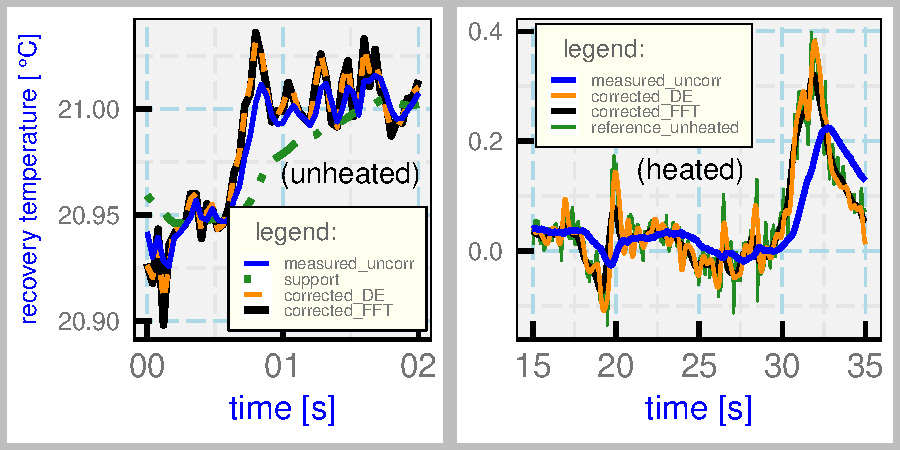
\includegraphics[width=12cm,height=5cm]{figure/figA1} \end{center}
\caption{Examples of the corrected recovery temperatures compared to the original uncorrected measurements. In each case, the correction based on the differential equations is shown as "corrected\_DE" and that based on Fourier transforms is labelled "corrected\_FFT." The dashed green line in the left plot shows the calculated temperature of the support that contacts the sensing wire. The solid green line in the right plot shows the corrected measurement from the unheated sensor for comparison. (left): An unheated sensor. Measurements from VOCALS flight 3. (right): A heated sensor. In this case the "corrected\_DE" result is based on Eq.\ \eqref{eq:HARCOsoln} while "corrected\_FFT" uses the fit provided by Eq.\ \eqref{eq:lfitH}. Mean values have been subtracted to facilitate comparison.\label{fig:sampleFFT}}
\end{figure}

If the response of the sensor is indeed linear, as the differential
equations indicate, a correction procedure equivalent to that described
above is first to filter the dynamic-heating term as in Sect.~3, correct
the measured recovery temperature by subtracting this filtered term, and
then apply one of the correction procedures described above to obtain
the corrected air temperature.



\codedataavailability{The data files used in this analysis are curated
as indicated by the following references and are publicly available.
They can be requested from the National Center for Atmospheric Research,
Earth Observing Laboratory, at this web site:
\href{https://data.eol.ucar.edu}{https://data.eol.ucar.edu}. The files
with references are as follows:

\begin{center}
\begin{tabular}{|c|c|}
\hline 
Research Project & Citation (see References)\tabularnewline
\hline 
\hline 
VOCALS & \citet{VOCALS2011}\tabularnewline
\hline 
CSET & \citet{CSET2017}\tabularnewline
\hline 
SOCRATES & \citet{SOCRATES2019}\tabularnewline
\hline 
\end{tabular}
\par\end{center}

This document is constructed in ways that support duplication of the
study. The code that generates the plots and implements the correction
procedure is incorporated into the same file that generated this
document via \LaTeX, using principles and techniques described by
\citet{Xie2015} as implemented in the R package ``knitr''
\citep{Xie2021}. The program, ``SensibleHeatFluxAMT.Rmd'' is archived on
``GitHub'' in the directory at
\href{https://github.com/WilliamCooper/SensibleHeatFlux.git}{this URL}.
There is some supplemental material in that directory, including a
workflow document and some code segments saved in the ``chunks''
subdirectory. The full directory should be downloaded in order to run
the program. The calculations use the programming language R
\citep{Rlanguage} and were run within RStudio \citep{RStudio2021}. A
package named Ranadu \citep{Ranadu2.6}, containing auxillary functions,
was used extensively in the R code and can be downloaded from that
reference.} %% use this section when having data sets and software code available



%%%%%%%%%%%%%%%%%%%%%%%%%%%%%%%%%%%%%%%%%%
%% optional

%%%%%%%%%%%%%%%%%%%%%%%%%%%%%%%%%%%%%%%%%%

%%%%%%%%%%%%%%%%%%%%%%%%%%%%%%%%%%%%%%%%%%
\authorcontribution{The first author wrote the processing code and
developed the general idea for the paper. The second author contributed
significantly to the manuscript and the presentation, and the third
author provided Laplace-transform solutions and a digital filter based
on them while also contributing to the
presentation.} %% optional section

%%%%%%%%%%%%%%%%%%%%%%%%%%%%%%%%%%%%%%%%%%
\competinginterests{The authors declare no competing
interests.} %% this section is mandatory even if you declare that no competing interests are present

%%%%%%%%%%%%%%%%%%%%%%%%%%%%%%%%%%%%%%%%%%

%%%%%%%%%%%%%%%%%%%%%%%%%%%%%%%%%%%%%%%%%%
\begin{acknowledgements}
This material is based upon work supported by the National Center for
Atmospheric Research, which is a major facility sponsored by the
National Science Foundation under Cooperative Agreement No.~1852977. The
data were collected using NSF's Lower Atmosphere Observing Facilities,
which are managed and operated by NCAR's Earth Observing Laboratory.
Measurements used here (\citet{VOCALS2011}, \citet{SOCRATES2019},
\citet{WECAN2018}) were collected in research projects
(\citet{wood2011vamos}, \citet{albrecht2019CSET},
\citet{mcfarquhar2021observations}) that used the NSF/NCAR research
aircraft. Project descriptions and additional information are available
at the EOL data site:
\href{https://data.eol.ucar.edu}{https://data.eol.ucar.edu}. The
referenced project teams conducted the experiments, with flight
operations, data acquisition and processing, and other project support
by the Research Aviation Facility, Earth Observing Laboratory, National
Center for Atmospheric Research (NCAR). The analyses reported here were
mostly performed using R (\citet{Rlanguage}), with RStudio
(\citet{RStudio2021}) and knitr (\citet{Xie2015,Xie2021}). Data files in
netCDF format have been read and written using the R package ``ncdf4''
(\citet{ncdf4}). Substantial use also was made of the ``ggplot2''
package (\citet{wickham2009}) for R, and extensive use was made of the
``stats'' package, part of Core R. Some of the numerical integrations
used the Runge-Kutta function from the ``rmutil'' package
(\citet{runge.kutta}). The Copernicus template provided by Daniel Nüst,
which uses the ``rticles'' package for R (\citet{rticles}), was used
with ``RMarkdown'' (\citet{XieEtAl2018RMarkdown}) to generate this
paper.
\end{acknowledgements}

%% REFERENCES
%% DN: pre-configured to BibTeX for rticles

%% The reference list is compiled as follows:
%%
%% \begin{thebibliography}{}
%%
%% \bibitem[AUTHOR(YEAR)]{LABEL1}
%% REFERENCE 1
%%
%% \bibitem[AUTHOR(YEAR)]{LABEL2}
%% REFERENCE 2
%%
%% \end{thebibliography}

%% Since the Copernicus LaTeX package includes the BibTeX style file copernicus.bst,
%% authors experienced with BibTeX only have to include the following two lines:
%%
\bibliographystyle{copernicus}
\bibliography{WAC.bib}
%%
%% URLs and DOIs can be entered in your BibTeX file as:
%%
%% URL = {http://www.xyz.org/~jones/idx_g.htm}
%% DOI = {10.5194/xyz}


%% LITERATURE CITATIONS
%%
%% command                        & example result
%% \citet{jones90}|               & Jones et al. (1990)
%% \citep{jones90}|               & (Jones et al., 1990)
%% \citep{jones90,jones93}|       & (Jones et al., 1990, 1993)
%% \citep[p.~32]{jones90}|        & (Jones et al., 1990, p.~32)
%% \citep[e.g.,][]{jones90}|      & (e.g., Jones et al., 1990)
%% \citep[e.g.,][p.~32]{jones90}| & (e.g., Jones et al., 1990, p.~32)
%% \citeauthor{jones90}|          & Jones et al.
%% \citeyear{jones90}|            & 1990


\end{document}
